\documentclass{training}
\schoollogo{../../resources/intros/UI-01-atomic-design.jpg}
\setlang{french}
\newcommand{\uxfond}{../../resources/fond/UI-01-atomic-design.png}
% Filigrane PAR MODULE : \uxfond (PNG A4 dilue 30 %). Cadre noir vectoriel commun.
% Proportions original 744 px : marge 20/744, trait 1/744. Exterieur BLANC.
% Cadre via eso-pic +\put (coordonnees absolues) — pas de remember picture (decalage).
\usepackage{eso-pic}

\providecommand{\uxfond}{../../resources/fond/norme_fond_paliers_30.png}

\newlength{\uxmargin}
\newlength{\uxthick}
\newlength{\uxinnerw}
\newlength{\uxinnerh}
\setlength{\uxmargin}{0.02688\paperwidth}% 20/744
\setlength{\uxthick}{0.001344\paperwidth}% 1/744
\setlength{\uxinnerw}{\dimexpr\paperwidth-2\uxmargin-2\uxthick\relax}
\setlength{\uxinnerh}{\dimexpr\paperheight-2\uxmargin-2\uxthick\relax}

% Contenu strictement a l'interieur du trait (+ jour confortable).
\geometry{%
  includeheadfoot,
  left=22mm,
  right=22mm,
  top=20mm,
  bottom=18mm,
  headheight=30pt,
  headsep=5mm,
  footskip=12mm%
}

\AddToShipoutPictureBG{%
  \AtPageLowerLeft{%
    % Fond blanc page entiere
    \put(0,0){\color{white}\rule{\paperwidth}{\paperheight}}%
    % Filigrane module a l'interieur du cadre
    \put(\LenToUnit{\dimexpr\uxmargin+\uxthick\relax},\LenToUnit{\dimexpr\uxmargin+\uxthick\relax}){%
      \includegraphics[width=\uxinnerw,height=\uxinnerh]{\uxfond}}%
    % Cadre noir : bas, haut, gauche, droite
    \put(\LenToUnit{\uxmargin},\LenToUnit{\uxmargin}){%
      \color{black}\rule{\dimexpr\paperwidth-2\uxmargin\relax}{\uxthick}}%
    \put(\LenToUnit{\uxmargin},\LenToUnit{\dimexpr\paperheight-\uxmargin-\uxthick\relax}){%
      \color{black}\rule{\dimexpr\paperwidth-2\uxmargin\relax}{\uxthick}}%
    \put(\LenToUnit{\uxmargin},\LenToUnit{\uxmargin}){%
      \color{black}\rule{\uxthick}{\dimexpr\paperheight-2\uxmargin\relax}}%
    \put(\LenToUnit{\dimexpr\paperwidth-\uxmargin-\uxthick\relax},\LenToUnit{\uxmargin}){%
      \color{black}\rule{\uxthick}{\dimexpr\paperheight-2\uxmargin\relax}}%
  }%
}

\makeatletter
\fancyhf{}
\fancyheadoffset{0pt}
\renewcommand{\headrulewidth}{0pt}
\lhead{\parbox[t]{0.56\textwidth}{\RaggedRight\footnotesize\sloppy\@title}}
\rhead{\parbox[t]{0.36\textwidth}{\RaggedLeft\footnotesize\sloppy\@subtitle}}
\cfoot{\thepage}
% Coupures : underscore et slash dans les noms de fichiers / consignes
\DeclareRobustCommand{\_}{\textunderscore\allowbreak}
\makeatother

% Evite les depassements de longues lignes (Github, Name_FirstName_...)
\sloppy
\emergencystretch=3em
\hbadness=10000

% Sommaire type 42 : chapitres seulement
\setcounter{tocdepth}{0}
\renewcommand{\cftchappresnum}{}
\renewcommand{\cftchapaftersnum}{}
\setlength{\cftchapnumwidth}{2.0em}
\setlength{\cftbeforechapskip}{0.35em}
\cftsetindents{chapter}{0em}{2.0em}


\begin{document}

\title{Design atomique}
\subtitle{Piscine UX/UI --- UI}
\member{Piscine UX/UI}{https://github.com/01-edu/UX-UI}
\summary{D'une revue de systèmes à deux bibliothèques qui ont un métier.}
\version{1.0}
\prerequisite{Le module précédent de cette piscine, ou aucun si c'est le premier.}
\maketitle

\newpage
\tableofcontents
\newpage


\chapter{Instructions}

L'avant-propos n'est pas un exercice. Il ne sera pas noté. Les exercices commencent au chapitre suivant, du contrat le plus simple au plus dur. Un exercice plus tardif n'est pas pris en compte si un plus tôt ne tient pas.

On ne regarde que ce qui est dans le répertoire de rendu de l'exercice. N'ajoutez pas un fichier que l'exercice ne nomme pas. Le nom d'un livrable suit le motif imprimé dans l'exercice : \texttt{Name\_FirstName\_DeliverableName\_Date\_VersionNumber}.

Le geste ne vous est pas donné. Les exemples d'un exercice portent parfois une contrainte que la phrase ne répète pas. Lisez-les. Vos autres références sont le manuel de l'outil choisi, la personne assise à côté, et les liens imprimés dans l'exercice.

L'ordre est celui de la quête. Sauter une étape parce qu'un écran plus tard semble plus intéressant produit un écran que personne ne sait expliquer.

\subsection*{Des images}

La marque en couverture est l'image de ce module. Les paliers pâles derrière le texte sont le fond de page. Ni l'un ni l'autre n'est un indice.

\subsection*{Des machines qui écrivent}

Vous pouvez vous servir d'un outil pour vérifier un mot, comme d'un dictionnaire. Vous ne pouvez pas remplacer un entretien, un test ou un fichier par un texte généré et le signer. Si vous ne pouvez pas montrer la personne, l'écran ou la ligne que vous avancez, l'exercice n'est pas fait.


\chapter{Avant-propos}

Brad Frost a nommé l'échelle atome, molécule, organisme, gabarit, page, et a mis l'essai en ligne (\url{https://atomicdesign.bradfrost.com/}). C'est un vocabulaire, comme une page de manuel est un vocabulaire. Appeler un bouton un atome ne dessine pas la bibliothèque.

\begin{center}
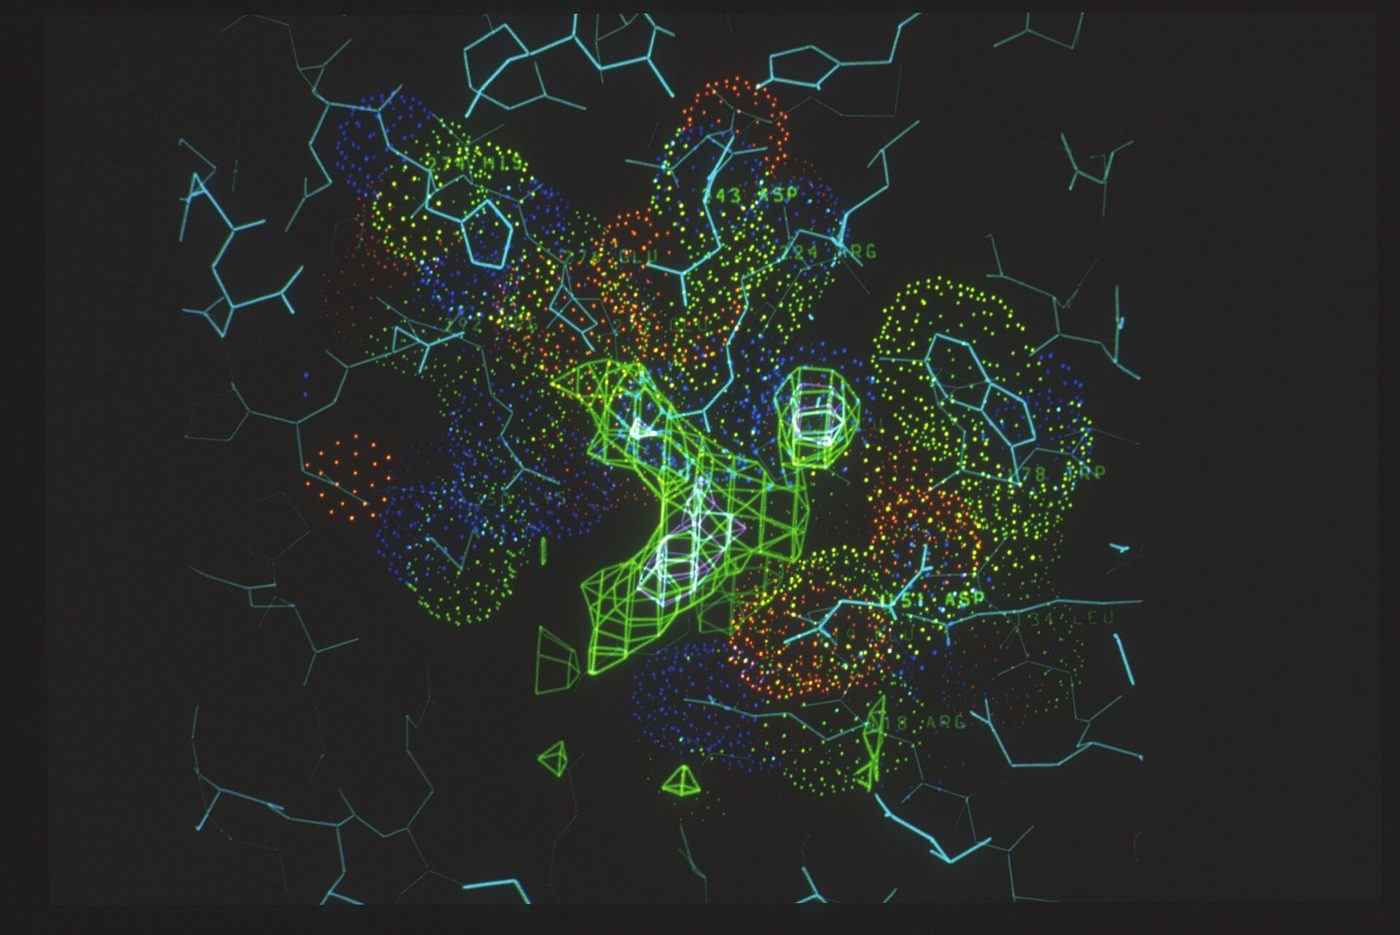
\includegraphics[width=0.78\textwidth,height=0.32\textheight,keepaspectratio]{../../resources/intros/UI-01-atomic-design.jpg}\\[0.4em]
{\footnotesize Image : division, CSIRO, CC BY 3.0}
\end{center}

À regarder. Les vidéos sont un contexte. Elles ne sont pas le livrable.
\begin{itemize}
\item UI - Introduction \& Quest n°1, 01Edu \url{https://www.youtube.com/watch?v=UbE6WMeuvQg&list=PLHyAJ_GrRtf-_aBft2jQL4-QAunn2bLvu}
\end{itemize}

\chapter{Exercice 00 : UI II - Ex 1 - Exploration}
\exnumber{00}
\extitle{UI II - Ex 1 - Exploration}
\exfiles{ex00/fichier Figma, nomme Name\_FirstName\_DeliverableName\_Date\_VersionNumber}
\exauthorize{Those named in the exercise}
\makeheaderfiles

\textbf{Contexte :}

Welcome to the 2nd quest of UI!

This series of exercises is a great occasion for you to discover how libraries are made in UI, thanks to Atomic Design.

\textbf{Instructions :}

Among these 4 websites, make snapshots of these elements:

\begin{itemize}
\item 1 template
\item 1 organism
\item 1 molecule
\item 1 atom
\end{itemize}

\textbf{Websites:}

\begin{itemize}
\item Alibaba
\item Booking.com
\item Easyjet App
\item Interrail
\end{itemize}

\textbf{Livrables :}

\begin{itemize}
\item A Figma file of 4 pages
\item On each page, a screenshot of a template, an organism, a molecule and an atom
\item Déposez le fichier Figma sur Github, nommé ainsi : « Name\_FirstName\_DeliverableName\_Date\_VersionNumber ». Exemple : « Doe\_John\_MidFiPrototype\_05242024\_V1 ».
\item Ajoutez un titre dans le fichier.
\item Soignez l'aspect global du fichier. Il doit être clair, simple et lisible. Vous pouvez regarder canva.com, sans surcharger le dessin de détails.
\end{itemize}

\textbf{Ressources :}

\begin{itemize}
\item Atomic Design Methodology \url{https://atomicdesign.bradfrost.com/chapter-2/}
\item Video tutorial on Figma \url{https://www.youtube.com/watch?v=FTFaQWZBqQ8}
\item Beginning graphic design \url{https://edu.gcfglobal.org/en/beginning-graphic-design/}
\item Gareth graphic studio \url{https://www.youtube.com/c/GarethDavidStudio}
\item Example here \url{https://www.figma.com/file/fzqDkk8Zc8qJCiSMbKV0Ei/UI-II---Ex-1?node-id=0%3A1}
\end{itemize}

\textbf{Citation :}

\begin{itemize}
\item User Interface Design is a hybrid role and can bring together concepts from interaction design, visual design, information architecture and even Front End Development
\end{itemize}


\chapter{Exercice 01 : UI II - Ex 2 - Material Design}
\exnumber{01}
\extitle{UI II - Ex 2 - Material Design}
\exfiles{ex01/fichier Figma, nomme Name\_FirstName\_DeliverableName\_Date\_VersionNumber}
\exauthorize{Ceux nommés dans l'exercice}
\makeheaderfiles

\textbf{Instructions :}

Téléchargez cette image \url{https://storage.googleapis.com/gd-wagtail-prod-assets/original_images/MDA2018_inline_02.jpg} qui est un aperçu de 3 écrans de Lyft, et détectez l'ordre dans lequel les calques ont été posés.

\textbf{Livrables :}

\begin{itemize}
\item Un fichier Figma avec l'image
\item Sur chaque écran, indiquer l'ordre des calques avec des numéros. 1 étant l'image de fond, 2 l'élément juste au-dessus, etc.
\item Déposez le fichier Figma sur Github, nommé ainsi : « Name\_FirstName\_DeliverableName\_Date\_VersionNumber ». Exemple : « Doe\_John\_MidFiPrototype\_05242024\_V1 ».
\item Ajoutez un titre dans le fichier.
\item Soignez l'aspect global du fichier. Il doit être clair, simple et lisible. Vous pouvez regarder canva.com, sans surcharger le dessin de détails.
\end{itemize}

\textbf{Pistes :}

\begin{itemize}
\item 2 chiffres peuvent être intervertis tant que l'ordre des calques est respecté
\end{itemize}

\textbf{Ressources :}

\begin{itemize}
\item Material Design Awards 2019 \url{https://design.google/library/material-design-awards-2019/}
\item Qu'est-ce que Material Design - Wikipedia \url{https://en.wikipedia.org/wiki/Material_Design}
\end{itemize}


\chapter{Exercice 02 : UI II - Ex 3 - Bibliothèque de design system}
\exnumber{02}
\extitle{UI II - Ex 3 - Bibliothèque de design system}
\exfiles{ex02/fichier Figma, nomme Name\_FirstName\_DeliverableName\_Date\_VersionNumber}
\exauthorize{Ceux nommés dans l'exercice}
\makeheaderfiles

\textbf{Instructions :}

Copiez 10 éléments du design system easyJet, incluant

\begin{itemize}
\item atoms
\item molecules
\item organisms
\end{itemize}

\textbf{Livrable :}

\begin{itemize}
\item Un fichier Figma comprenant 10 éléments du design system easyJet
\item Déposez le fichier Figma sur Github, nommé ainsi : « Name\_FirstName\_DeliverableName\_Date\_VersionNumber ». Exemple : « Doe\_John\_MidFiPrototype\_05242024\_V1 ».
\item Ajoutez un titre dans le fichier.
\item Soignez l'aspect global du fichier. Il doit être clair, simple et lisible. Vous pouvez regarder canva.com, sans surcharger le dessin de détails.
\end{itemize}

\textbf{Pistes :}

\begin{itemize}
\item Vous pouvez utiliser Avenir Book à la place de la police d'easyJet
\item Explorer Noun Project pour trouver des icônes
\end{itemize}

\textbf{Ressources :}

\begin{itemize}
\item Méthodologie Atomic Design \url{https://atomicdesign.bradfrost.com/chapter-2/}
\end{itemize}


\chapter{Exercice 03 : UI II - Ex 4 - Bibliothèque pour grimpeurs}
\exnumber{03}
\extitle{UI II - Ex 4 - Bibliothèque pour grimpeurs}
\exfiles{ex03/fichier Figma, nomme Name\_FirstName\_DeliverableName\_Date\_VersionNumber}
\exauthorize{Ceux nommés dans l'exercice}
\makeheaderfiles

\textbf{Instructions :}

Vous faites partie d'un groupe d'escalade et vous vous portez volontaire pour rebrander le site web de votre club.

À partir d'un moodboard, créez un design system avec au moins 20 éléments, incluant atoms, molecules et organisms, et incluez des multistates.

\textbf{Livrables :}

\begin{itemize}
\item Un fichier Figma avec une planche d'ambiance pour un groupe d'escalade. Incluez :
\begin{itemize}
\item Des photos
\item Couleurs (2 à 3 couleurs principales)
\item Typographie
\end{itemize}
\item Un fichier Figma avec une bibliothèque comprenant :
\begin{itemize}
\item Au moins 20 éléments de design graphique
\item Au moins un atome
\item Au moins une molécule
\item Au moins un organisme
\item Au moins 5 éléments multi-états
\end{itemize}
\item Déposez les documents sur Github, dans un zip nommé « ProjectTitle\_Name\_FirstName », et chaque livrable ainsi : « Name\_FirstName\_DeliverableName\_Date\_VersionNumber ». Exemple : « Doe\_John\_MidFiPrototype\_05242024\_V1 ».
\item Ajoutez un titre dans tous les documents écrits.
\item Soignez l'aspect global des livrables. Ils doivent être clairs, simples et lisibles. Vous pouvez regarder canva.com, sans surcharger le dessin de détails.
\end{itemize}

\textbf{Pistes :}

\begin{itemize}
\item Soyons créatifs ! Inspirez-vous de visuels avant de vous lancer.
\item Inspirez-vous des design systems existants. Parcourez Dribbble et la communauté Figma.
\end{itemize}

\textbf{Ressources :}

\begin{itemize}
\item Introduction aux design systems \url{https://www.youtube.com/watch?v=xEuBCUngJ_U}
\item Créer un design system - cours Figma \url{https://www.youtube.com/watch?v=RYDiDpW2VkM}
\item Construire une library de design system - Lyft \url{https://medium.com/tap-to-dismiss/building-a-design-system-library-532ef2492811}
\item Exemples de library de boutons UI \url{https://www.pinterest.co.kr/pin/663014376380850291/}
\end{itemize}


\chapter{Exercice 04 : UI II - Ex 5 - Bibliothèque pour une application de rencontre}
\exnumber{04}
\extitle{UI II - Ex 5 - Bibliothèque pour une application de rencontre}
\exfiles{ex04/fichier Figma, nomme Name\_FirstName\_DeliverableName\_Date\_VersionNumber}
\exauthorize{Ceux nommés dans l'exercice}
\makeheaderfiles

\textbf{Instructions :}

On vous demande de concevoir une application de rencontre.

À partir d'un moodboard que vous avez composé, créez un design system avec au moins 20 éléments, incluant atoms, molecules et organisms, et incluez des multistates.

\textbf{Livrables :}

\begin{itemize}
\item Un fichier Figma avec une planche d'ambiance pour une application de rencontre. Incluez :
\begin{itemize}
\item Des photos
\item Couleurs (2 à 3 couleurs principales)
\item Typographie
\end{itemize}
\item Un fichier Figma avec une bibliothèque comprenant
\begin{itemize}
\item Au moins 20 éléments de design graphique
\item Au moins un atome
\item Au moins une molécule
\item Au moins un organisme
\item Au moins 5 éléments multi-états
\end{itemize}
\item Déposez les documents sur Github, dans un zip nommé « ProjectTitle\_Name\_FirstName », et chaque livrable ainsi : « Name\_FirstName\_DeliverableName\_Date\_VersionNumber ». Exemple : « Doe\_John\_MidFiPrototype\_05242024\_V1 ».
\item Ajoutez un titre dans tous les documents écrits.
\item Soignez l'aspect global des livrables. Ils doivent être clairs, simples et lisibles. Vous pouvez regarder canva.com, sans surcharger le dessin de détails.
\end{itemize}

\textbf{Pistes :}

\begin{itemize}
\item Soyons créatifs ! Inspirez-vous de visuels avant de vous lancer.
\item Inspirez-vous des design systems existants. Parcourez Dribbble et la communauté Figma.
\end{itemize}

\textbf{Ressources :}

\begin{itemize}
\item Introduction aux design systems \url{https://www.youtube.com/watch?v=xEuBCUngJ_U}
\item Créer un design system - cours Figma \url{https://www.youtube.com/watch?v=RYDiDpW2VkM}
\item Construire une library de design system - Lyft \url{https://medium.com/tap-to-dismiss/building-a-design-system-library-532ef2492811}
\item Exemples de library de boutons UI \url{https://www.pinterest.co.kr/pin/663014376380850291/}
\end{itemize}


\end{document}
